%% 
%% Copyright 2007-2025 Elsevier Ltd
%% 
%% This file is part of the 'Elsarticle Bundle'.
%% ---------------------------------------------
%% 
%% It may be distributed under the conditions of the LaTeX Project Public
%% License, either version 1.3 of this license or (at your option) any
%% later version.  The latest version of this license is in
%%    http://www.latex-project.org/lppl.txt
%% and version 1.3 or later is part of all distributions of LaTeX
%% version 1999/12/01 or later.
%% 
%% The list of all files belonging to the 'Elsarticle Bundle' is
%% given in the file `manifest.txt'.
%% 
%% Template article for Elsevier's document class `elsarticle'
%% with numbered style bibliographic references
%% SP 2008/03/01
%% $Id: elsarticle-template-num.tex 272 2025-01-09 17:36:26Z rishi $
%%
%%\documentclass[preprint,12pt]{elsarticle}
\documentclass[times, review, 10pt]{elsarticle}

%% Use the option review to obtain double line spacing
%% \documentclass[authoryear,preprint,review,12pt]{elsarticle}

%% Use the options 1p,twocolumn; 3p; 3p,twocolumn; 5p; or 5p,twocolumn
%% for a journal layout:
%% \documentclass[final,1p,times]{elsarticle}
%% \documentclass[final,1p,times,twocolumn]{elsarticle}
%% \documentclass[final,3p,times]{elsarticle}
%% \documentclass[final,3p,times,twocolumn]{elsarticle}
%% \documentclass[final,5p,times]{elsarticle}
%% \documentclass[final,5p,times,twocolumn]{elsarticle}

%% For including figures, graphicx.sty has been loaded in
%% elsarticle.cls. If you prefer to use the old commands
%% please give \usepackage{epsfig}

%% The amssymb package provides various useful mathematical symbols
\usepackage{amssymb}
%% The amsmath package provides various useful equation environments.
\usepackage{amsmath,amsfonts}
%% The amsthm package provides extended theorem environments
%% \usepackage{amsthm}

%% The lineno packages adds line numbers. Start line numbering with
%% \begin{linenumbers}, end it with \end{linenumbers}. Or switch it on
%% for the whole article with \linenumbers.
%% \usepackage{lineno}

\usepackage{algorithmic}
\usepackage{algorithm}
\usepackage{array}
\usepackage[caption=false,font=normalsize,labelfont=sf,textfont=sf]{subfig}
\usepackage{xcolor}
\usepackage{textcomp}
\usepackage{stfloats}
\usepackage{url}
\usepackage{verbatim}
\usepackage{graphicx}
\usepackage{comment}

% Recommended, but optional, packages for figures and better typesetting:
\usepackage{microtype}
\usepackage{booktabs} % for professional tables
\usepackage{tabularx}

% For theorems and such
\usepackage{amssymb}
\usepackage{mathtools}
\usepackage{amsthm}
\usepackage{comment}

\usepackage{bm}             % math notation
\usepackage{bbm}            % math notation
\usepackage{multirow}
\usepackage{enumitem}

\journal{Pattern Recognition}

\begin{document}

\begin{frontmatter}

%% Title, authors and addresses

%% use the tnoteref command within \title for footnotes;
%% use the tnotetext command for theassociated footnote;
%% use the fnref command within \author or \affiliation for footnotes;
%% use the fntext command for theassociated footnote;
%% use the corref command within \author for corresponding author footnotes;
%% use the cortext command for theassociated footnote;
%% use the ead command for the email address,
%% and the form \ead[url] for the home page:
%% \title{Title\tnoteref{label1}}
%% \tnotetext[label1]{}
%% \author{Name\corref{cor1}\fnref{label2}}
%% \ead{email address}
%% \ead[url]{home page}
%% \fntext[label2]{}
%% \cortext[cor1]{}
%% \affiliation{organization={},
%%             addressline={},
%%             city={},
%%             postcode={},
%%             state={},
%%             country={}}
%% \fntext[label3]{}

\title{Concrete Dense Network for Long-Sequence Time Series Clustering} %% Article title

%% use optional labels to link authors explicitly to addresses:
%% \author[label1,label2]{}
%% \affiliation[label1]{organization={},
%%             addressline={},
%%             city={},
%%             postcode={},
%%             state={},
%%             country={}}
%%
%% \affiliation[label2]{organization={},
%%             addressline={},
%%             city={},
%%             postcode={},
%%             state={},
%%             country={}}

\author[label1]{Redemptor Jr Laceda Taloma} %% Author name
\author[label2]{Patrizio Pisani}
\author[label1]{Danilo Comminiello}

%% Author affiliation
\affiliation[label1]{organization={Department of Information Engineering, Electronics and Telecommunications,\\ Sapienza University of Rome},
            addressline={Via Eudossiana 18},
            city={Rome},
            postcode={00184},
            country={Italy}}

\affiliation[label2]{organization={Unidata S.p.A.},
            addressline={Viale A. G. Eiffel 100},
            city={Rome},
            postcode={00148},
            country={Italy}}

\begin{abstract}
Time series clustering is fundamental in data analysis for discovering temporal patterns. Despite recent advancements, learning cluster-friendly representations is still challenging, particularly with long and complex time series. Deep temporal clustering methods have been trying to integrate the canonical \textit{k}-means into end-to-end training of neural networks but fall back on surrogate losses due to the non-differentiability of the hard cluster assignment, yielding sub-optimal solutions. In addition, the autoregressive strategy used in the state-of-the-art RNNs is subject to error accumulation and slow training, while recent research findings have revealed that Transformers are less effective due to time points lacking semantic meaning, to the permutation invariance of attention that discards the chronological order and high computation cost.
In light of these observations, we present LoSTer, which is a novel dense autoencoder architecture for \textcolor{blue}{long-sequence time series clustering (LSTC)} capable of optimizing the \textit{k}-means objective via the Gumbel-softmax reparameterization trick and designed specifically for accurate and fast clustering of long time series. Extensive experiments on numerous benchmark datasets and two real-world applications prove the effectiveness of LoSTer over state-of-the-art RNNs and Transformer-based deep clustering methods.
\end{abstract}

%%Graphical abstract
%\begin{graphicalabstract}
%\includegraphics{grabs}
%\end{graphicalabstract}

%%Research highlights
\begin{comment}
\begin{highlights}
\item We present the first deep learning method for time series clustering that optimizes the \textit{k}-means objective without falling back to sub-optimal surrogates, which cause inconsistent assignments in existing solutions.
\item Moving from the solid findings of the long-term time series forecasting research, this work provides empirical discussions on the poor capacity of state-of-the-art Transformers in performing long-sequence time series clustering.
\item A novel and simple yet effective dense autoencoder is designed specifically for long-sequence time series clustering, overcoming the current limitations of RNNs and Transformers.
\item The proposed model boasts significant training speedup to RNNs and Transformer-based competitors when applied to large-scale datasets.
\end{highlights}
\end{comment}

%% Keywords
\begin{keyword}
clustering \sep time series \sep machine learning \sep deep learning
\end{keyword}


\end{frontmatter}

%% Add \usepackage{lineno} before \begin{document} and uncomment 
%% following line to enable line numbers
%% \linenumbers

%% main text
%%

\section{Introduction}
Clustering is relevant for time series analysis in many applications as it helps discover temporal patterns from unlabeled data \cite{liao2005clustering,lee2024deep}. However, the widespread collection of increasingly longer time series data collected by sensors unveils the limits of current solutions \cite{el2023constrained}. New challenges posed by long-sequence time series clustering (LSTC) emerge from the need to design temporal clustering algorithms that can effectively handle high dimensionality and achieve computational scalability when applied to large-scale datasets \cite{li2021multivariate}.

The \textit{k}-means algorithm is a straightforward and informative method to group data with high similarity within clusters, including time series \cite{yang2017towards,zhang2025structured}. However, the assumption of underlying spherical cluster distribution causes poor performance when time series exhibit non-linear dynamics, particularly if spanning over thousands of time steps. Therefore, unsupervised learning of feature spaces for clustering is nowadays an active area of research \cite{ren2025deep}.

Rather than original data, feature-based methods cluster lower-dimensional representations to filter irrelevant information and reduce noise and outliers. However, these methods require domain expertise to handcraft such features properly. In light of this, deep learning has been proposed for shaping an \emph{ad hoc} latent space in which representation learning and clustering are simultaneously performed, leading to deep learning clustering. Deep Embedding for Clustering (DEC) \cite{xie2016unsupervised} emerged as the first joint optimization on static data (e.g. images): it defines a non-linear mapping parameterized by a neural network from the original to the latent space, where the clustering objective is optimized using gradient descent. The Improved Deep Embedding for Clustering (IDEC) \cite{guo2017improved} integrates a reconstruction term into DEC to preserve the local structure of the data, inspiring Madiraju et al. (2018) \cite{madiraju2018deep} to design Deep Temporal Clustering (DTC) as an extension of IDEC to time series thanks to a CNN-BiLSTM autoencoder performing spatiotemporal dimensionality reduction. The drawback, though, is DTC as well as DEC and IDEC refining clusters by minimizing the Kullback-Leibler divergence to an auxiliary target distribution based on the current soft cluster assignments, instead of the \textit{k}-means objective: this surrogate loss is known not to be sub-optimal and favours overlapping compared to hard clustering \cite{gao2020deep}.

Ma et al. (2019) \cite{ma2019learning} proposed Deep Temporal Clustering Representation (DTCR), which integrates time series reconstruction and \textit{k}-means to generate cluster-specific temporal representations through a Dilated RNN \cite{chang2017dilated}. Zhong et al. (2023) \cite{zhong2023deep} further include contrastive learning in their Deep Temporal Contrastive Clustering (DTCC), but neither DTCR nor DTCC is optimizing the canonical \textit{k}-means objective due to the \textcolor{blue}{non-differentiability} of the hard cluster assignment. Indeed, they seek to minimize a soft \textit{k}-means objective, which can be converted into a trace maximization problem via spectral relaxation \cite{zha2001spectral}. However, its implementation requires fixing the cluster assignments for a predefined number of iterations to avoid instability while updating data representations, possibly causing inconsistent assignments in mini-batch stochastic gradient descent. LSTC \textcolor{blue}{tasks} may require many iterations if the dataset is large, eventually making this phenomenon more detrimental.

Therefore, we design Long-Sequence Temporal Concrete Clustering (LoSTer) resulting in the first end-to-end deep learning model solving the \textcolor{blue}{non-differentiability} of the \textit{k}-means discrete cluster assignment of time series, by exploiting the Gumbel-softmax reparameterization trick \cite{jang2017categorical}.

Furthermore, LoSTer defines a simple and yet effective dense architecture to overcome 1) the limiting autoregressive single-layer RNN of DTCR and DTCC subject to error accumulation and slowing down training due to processing the observations in the sequence recursively and 2) the inadequacy of the point-wise attention mechanism in Transformers to capture temporal dependencies over long time series while also being hindered by quadratic computation cost and space requirements. The issues in Transformers, which are known findings from the long-term time series forecasting research \cite{zeng2023transformers}, are even exacerbated in LSTC because the aim is to cluster large batches of long time series as a whole rather than forecasting the future of each time series individually. Specifically, the high memory occupation caused by embedding each of the many temporal observations forces to set a smaller batch size: since deep clustering is performed batch-wise, smaller and therefore less representative batches cause a drop in performance. Conversely, linear models have shown in literature remarkable predictive capability in handling trends, seasonality and shifts in time series, while boasting higher efficiency \cite{zeng2023transformers,li2023revisiting}.

Experimental results on 17 long-sequence time series benchmark datasets show LoSTer outperforming state-of-the-art RNNs and Transformers in terms of clustering accuracy and training speed, thus eventually delivering a simple, fast to train and scalable method for LSTC. Moreover, superior performance on two more challenging large-scale retail datasets proves the effectiveness in real-world use cases. The main contributions of this work are summarized as follows:

\begin{enumerate}
    \item To the best of our knowledge in time series clustering, LoSTer is the first deep learning model that optimizes the \textit{k}-means objective without falling back to sub-optimal surrogates. Unlike DTCR and DTCC, cluster assignments are not fixed for a predefined number of iterations, avoiding inconsistent assignments.
    \item Moving from the solid findings of the \textcolor{blue}{long-term} time series forecasting research, this work provides empirical discussions on the poor capacity of state-of-the-art Transformers in performing LSTC.
    \item A novel dense autoencoder is designed specifically for LSTC, overcoming effectively the limitations of RNNs and Transformers.
    \item LoSTer boasts significant training speedup to RNNs and Transformer-based competitors when applied to large-scale datasets.
\end{enumerate}

\textcolor{blue}{The source code for the present study is available on GitHub}\footnote{\url{https://github.com/jrtaloma/lstc}}.

\section{Related Works}
In this section, we provide an overview of relevant literature based on different methodological paradigms.

\paragraph{Raw-based Methods} Time series clustering is divided into raw-based and feature-based methods. The traditional \textit{k}-means algorithm minimizes the square of intra-cluster Euclidean distance. When applied to time series, though, this metric is extremely restrictive because the time steps are matched point-wise. For this reason, raw-based methods are applied with a modified similarity measure. For example, \textit{k}-DBA \cite{petitjean2011global} uses Dynamic Time Warping (DTW) and performs clustering based on the aligned set of sequences. Similarly, K-Spectral Centroid (K-SC) \cite{yang2011patterns} clusters temporal sequences based on a similarity metric that is invariant to scaling and shifting. However, all raw-based methods are sensitive to noise and outliers because they involve every time step.

\paragraph{Feature-Based Methods} Instead of considering all time steps, feature-based methods reduce the data dimension to alleviate the impact of high-frequency noise, temporal gaps, and outliers. Examples include adaptive piece-wise constant approximation \cite{keogh2001locally}, nonnegative matrix factorization \cite{brockwell1991time}, and Independent Component Analysis (ICA) \cite{guo2008time}. However, these are two-stage approaches in which the dimensionality reduction and clustering are performed independently, causing the potential loss of temporal information.

\paragraph{Deep Temporal Clustering} The interest in time series deep clustering has grown due to the ability to learn a latent space that captures the properties of data without manual feature engineering. These models have also the benefit of jointly optimizing the feature extraction and clustering. DTC \cite{madiraju2018deep} uses an autoencoder and a clustering layer, trained by minimizing the Kullback-Leibler divergence between the predicted and target distribution. DTCR \cite{ma2019learning} incorporates the \textit{k}-means objective into the model via spectral relaxation. More recently, following the growing interest in contrastive learning for image clustering \cite{deng2023strongly,peng2022crafting}, DTCC \cite{zhong2023deep} has shown a novel dual contrastive learning approach yielding more informative discriminative features for time series clustering.

\paragraph{Learning Representation from Time Series} Regardless of their complicated self-attention scheme, a very simple linear model \cite{zeng2023transformers} has been able to outperform the state-of-the-art Transformers on a variety of common long-term time series forecasting benchmarks \cite{misc_electricityloaddiagrams20112014_321,lai2018modeling}. This remarks that designing an encoder that learns an effective representation of long time series is still an open challenge. In this work, we design a new dense architecture for time series clustering partly inspired by the Time-Series Dense Encoder (TiDE) \cite{daslong}, which achieves superior forecasting accuracy and faster computation when compared to a strong patch time series Transformer \cite{Yuqietal-2023-PatchTST}. Similarly, Preformer \cite{du2023preformer} and Pathformer \cite{chenpathformer} have recently proposed segment-wise and patch-level attention at multiple scales, respectively, to overcome the standard point-wise attention while also capturing different characteristics for various resolutions.

\section{Proposed Method}
\begin{figure}[!tb]
  \centering
  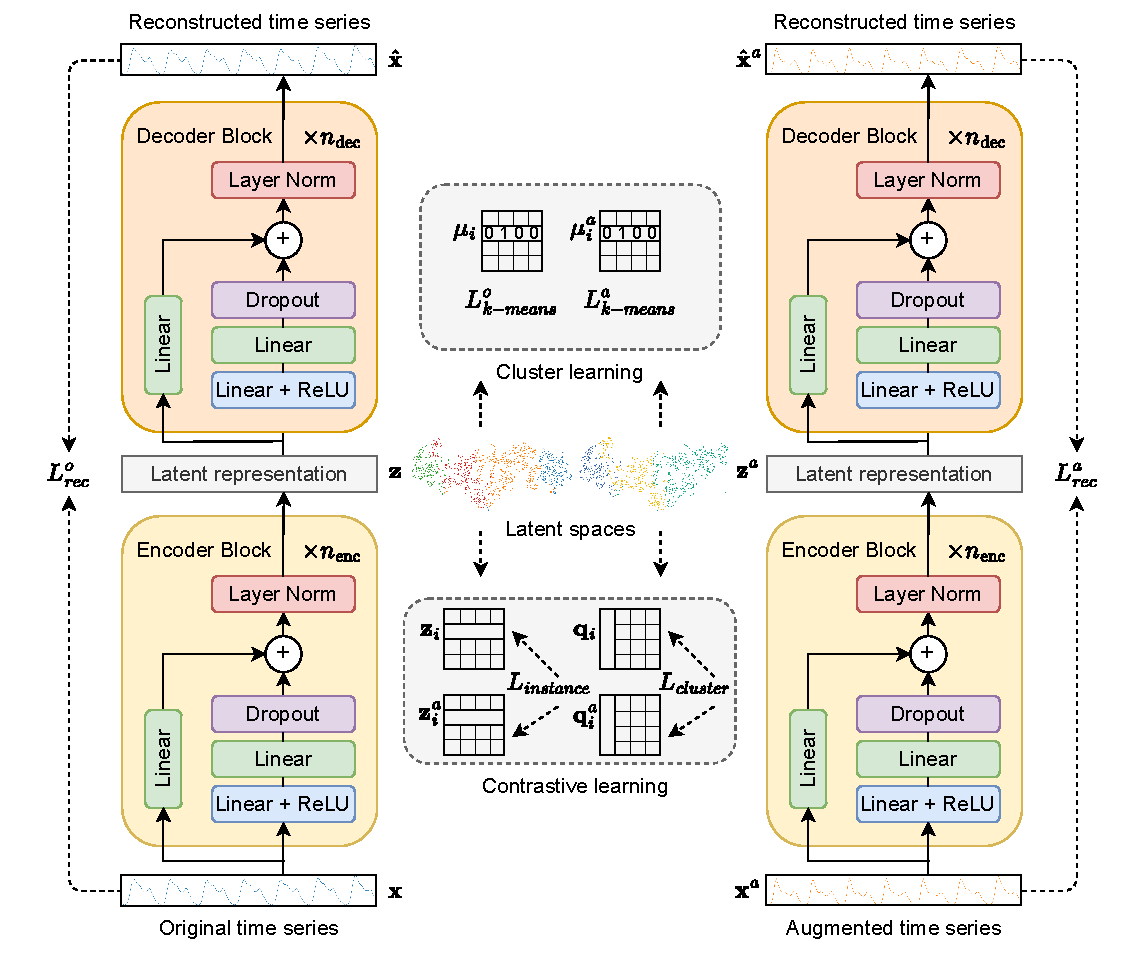
\includegraphics[width=\linewidth]{Figure_1.pdf}
  \caption{The overall architecture of LoSTer for long-sequence time series clustering (LSTC). It employs a two-view architecture with identical autoencoders for reconstructing original and augmented time series. Both the encoder and decoder are instantiated as a stack of dense residual blocks. The latent representations of data and centroids and the cluster assignments are learned end-to-end through \textit{k}-means and dual contrastive loss.}
  \label{fig:DenseAutoencoder}
\end{figure}

\textcolor{blue}{We presented} LoSTer, a novel deep-learning method for long-sequence time series clustering. Compared to current state-of-the-art DTCR and DTCC, LoSTer is not limited to producing cluster-friendly representations of time series but is also able to predict the final clusters end-to-end, hence without the need of performing \textit{k}-means on the latent representations at the end of the training process. A new dense encoder-decoder architecture and the optimization are described in this section. \textcolor{blue}{The architecture diagram is illustrated in Fig. \ref{fig:DenseAutoencoder}.}

\subsection{Preliminaries}
Consider a set of $n$ time series  $D = \{ \mathbf{x}_1, ..., \mathbf{x}_n \}$ where each ordered sequence $\mathbf{x}_i$ contains $L$ time steps and is denoted as $\mathbf{x}_i = [x_{i,1}, ..., x_{i,L}]$. Given a positive integer $k \leq n$, we perform \textit{k}-means clustering to partition the $n$ instances in $D$ into $k$ clusters.

\textcolor{blue}{Since this work relies on} a contrastive learning approach, we need to define an augmentation function $\textit{T}$. \textcolor{blue}{As proposed by Um et al. (2017) \cite{um2017data}, for each instance $\mathbf{x}_i$, we compute in advance its augmented version $\mathbf{x}_i^a = T(\mathbf{x}_i)$, where $T$ is the composition of rotation, permutation, and time-warping to perturb the temporal location of time series sensor data. For rotation, each time series $\mathbf{x}_i$ in the batch of data can be flipped or not by randomly drawing a sign flip from \{-1, 1\}. For permutation, a random integer $n_{splits}$ is determined by rounding a positive value sampled from a Gaussian distribution (mean = 0, std = 5.0); then, we slice the time series into $n_{splits}$ segments and randomly permute them. Time warping is applied by smoothly distorting the temporal axis of each time series using cubic spline interpolation, with scaling factors sampled from a Gaussian distribution (mean = 1.0, std = 0.2) at 6 control points along the time axis. Composing these augmentations alters the location of events and temporal progression.}

\subsection{Method Overview}
LoSTer employs a two-view architecture in which two identical autoencoders reconstruct the original and augmented time series while performing cluster learning in the corresponding latent spaces. The autoencoder is structured as a simple and efficient MLP-based architecture. The encoder is built as a stack of residual blocks mapping the input time series to a lower-dimensional feature vector. The decoder uses a similar stack to reconstruct the input sequence given the encoded representation. Meanwhile, exploiting the Gumbel-softmax reparameterization trick, the centroid representation matrix can be defined as a learnable parameter of the model, thus learned end-to-end without alternating with cluster assignments updates, as opposed to DTCR and DTCC. \textcolor{blue}{Following Li et al. (2021) \cite{li2021contrastive} and Zhong et al. (2023) \cite{zhong2023deep}, dual contrastive learning is enforced to take full advantage of the two-view architecture.}

\subsection{Dense Encoder-Decoder Architecture}
State-of-the-art solutions for time series clustering capture the temporal dynamics through the Dilated RNN, which extracts multi-scale features using dilated recurrent skip connections and exponentially increasing dilation. This multi-scale architecture improved the ability of recurrent models to learn time dependency. However, DTCR and DTCC still propose an autoregressive single-layer RNN as the decoder for reconstructing the input time series. This choice affects the reconstruction ability in the decoding phase because the autoregressive strategy is prone to error accumulation, particularly on longer sequences with intricate patterns.
To overcome this issue, we introduce a deep temporal clustering model featuring an MLP-based autoencoder architecture, whose decoder performs the reconstruction of the time series from the encoded representation using the multi-step direct strategy instead of autoregression.

\textbf{Residual Block.} The core component is a residual block with one hidden layer and a fully linear skip connection. Let $\mathbf{x}$ be the input vector to the module. The hidden layer with the ReLU activation function is followed by a linear transformation that maps the embedding $\mathbf{h}$ to the output representation $\mathbf{o}$. Dropout is enabled during training for regularization. Layer normalization is applied at the end. Formally:
%
\begin{equation}
\mathbf{h} = \text{ReLU}(\text{Linear}(\mathbf{x}))
\end{equation}
%
\begin{equation}
\mathbf{h'} = \text{Dropout}(\text{Linear}(\mathbf{h})) + \text{Linear}(\mathbf{x})
\end{equation}
%
\begin{equation}
\mathbf{o} = \text{LayerNorm}(\mathbf{h'})
\end{equation}
%
\textbf{Encoder.} The dense encoder \text{Enc} of LoSTer is a stack of $n_{\text{enc}}$ residual blocks mapping the input sequence $\mathbf{x}_i$ to a vector $\mathbf{z}_i$ in a $d$-dimensional latent space.
%
\begin{equation}
    \mathbf{z}_i = \text{Enc}(\mathbf{x}_i)
\end{equation}
%
\textbf{Decoder.} The dense decoder \text{Dec} is defined as a stack of $n_{\text{dec}}$ residual blocks with the same hidden size $d$ as the encoder, producing the reconstruction $\hat{x}_i$ of the input.
%
\begin{equation}
    \hat{x}_i = \text{Dec}(\mathbf{z}_i)
\end{equation}

\subsection{Deep Temporal Reconstruction with Parallel Views}
 We aim to learn two non-linear encoding transformations $f_{\text{enc}}: \mathbf{x}_i \rightarrow \mathbf{z}_i $ for the original view and $f_{\text{enc}}^a: \mathbf{x}_i^a \rightarrow \mathbf{z}_i^a $ for the augmented view, mapping the original and augmented sequence respectively into the latent space $\textit{Z}$ and $\textit{Z}^a$ $\subset \mathbb{R}^d$. Moreover, we define two non-linear decoding transformations $f_{\text{dec}}: \mathbf{z}_i \rightarrow \mathbf{\hat{x}}_i $ and $f_{\text{dec}}^a: \mathbf{z}_i^a \rightarrow \mathbf{\hat{x}}_i^a $ mapping the latent representations $\mathbf{z}_i$ and $\mathbf{z}_i^a$ back to the initial input space of each view. To capture the dynamics of time series, we instantiate the encoding and decoding functions $f_{\text{enc}}$ and  $f_{\text{dec}}$ as the encoder and decoder, respectively, of the proposed dense autoencoder described above. Similarly, the same classes of neural networks are instantiated for the functions $f_{\text{enc}}^a$ and $f_{\text{dec}}^a$ in the augmented view. Thus, the two autoencoders are identical but have different weights. To push the network to learn meaningful representations, we use the Mean Squared Error (MSE) as the reconstruction loss for training the encoder-decoder composition in each view. Formally:
%
\begin{equation}
    L_{rec}^o = \frac{1}{n} \sum_{i=1}^n \lvert\lvert \mathbf{x}_i - \mathbf{\hat{x}}_i \rvert\rvert_2^2
\end{equation}
%
\begin{equation}
    L_{rec}^a = \frac{1}{n} \sum_{i=1}^n \lvert\lvert \mathbf{x}_i^a - \mathbf{\hat{x}}_i^a \rvert\rvert_2^2
\end{equation}
%
Therefore, the joint reconstruction loss is:
%
\begin{equation}
    L_{rec} = L_{rec}^o + L_{rec}^a
\end{equation}

\subsection{Differentiable Discrete Clustering}
Though needed for consistency, the reconstruction loss is not purposed to capture cluster-level information. To this end, we describe a cluster distribution learning method capable of optimizing the hard-cluster assignment of the \textit{k}-means objective directly, enabling end-to-end gradient-based learning, and therefore without resorting to a soft \textit{k}-means relaxation as opposed to existing works.

In deep \textit{k}-means, the latent representations in the embedding space $\textit{Z}$ are partitioned into $\textit{k}$ different clusters. The optimization problem is to find the assignment and set of $\textit{k}$ centroids that minimize the sum of squared distances between each $\mathbf{z}_i$ and its associated centroid. Formally:
%
\begin{equation}
\min_{\mathbf{Q},\mathbf{M}} \lvert\lvert \mathbf{Z} - \mathbf{Q}\mathbf{M} \rvert\rvert_F^2 \text{ s.t. $\lvert\lvert \mathbf{q}_i \rvert\rvert_1 = 1$} \text{, $\mathbf{Q} \in \{0, 1\}^{n \times k}$}
\end{equation}
%
where the row $\mathbf{q}_i$ of the binary matrix $\mathbf{Q}$ is a one-hot encoding representing the assignment of $\mathbf{z}_i$ to one cluster only. $\mathbf{M} \in \mathbb{R}^{k \times d}$ is the centroid matrix, in which rows $\bm{\mu}_j$ are the centroid representations in the latent space.

The \textit{k}-means algorithm alternates the cluster assignments and cluster centers optimization until convergence. However, in deep \textit{k}-means clustering, backpropagation is not possible as the discrete cluster assignment is not differentiable. Therefore, we exploit the Gumbel-softmax reparameterization trick, which uses a stochastic hard assignment in the forward pass while allowing gradient backpropagation through the soft assignment. This enables the end-to-end training of the neural network.
%
\begin{equation}
    p(C_{i,j} | \mathbf{x}_i) = \frac{\exp{\{ -\sigma^{-2} \lvert\lvert \mathbf{z}_i - \bm{\mu}_j \rvert\rvert_2^2 \}}}{\sum_{c=1}^k \exp \{ -\sigma^{-2} \lvert\lvert \mathbf{z}_i - \bm{\mu}_c \rvert\rvert_2^2 \}}
    \label{rbf}
\end{equation}
%
As shown in Eq. \ref{rbf}, the cluster assignment probabilities are based on the Euclidean distance and modeled using the normalized radial basis function (RBF). Specifically, $p(C_{i,j} | \mathbf{x}_i)$ is the probability of the event that $\mathbf{x}_i$ is assigned to cluster $j$, whose centroid is $\bm{\mu}_j$, considering all the centroid distances of the corresponding representation $\mathbf{z}_i$. At this point, we use the reparameterization trick in Eq. \ref{gumbel} to draw samples $\mathbf{q}_i$ from a categorical distribution with class probabilities $p(C_{i,j} | \mathbf{x}_i)$ for $j \in \{1, ..., k\}$, while still being able to perform backpropagation through the sampling process.
%
\begin{equation}
    q_{i,j} = \frac{\exp{\{ (\log({p(C_{i,j} | \mathbf{x}_i)}) + g_j ) / \tau \}}}{\sum_{c=1}^k \exp{\{ (\log({p(C_{i,c} | \mathbf{x}_i)}) + g_c) / \tau \}} }
    \label{gumbel}
\end{equation}
%
Here $q_{i,j}$ is the \emph{j}-th entry of $\mathbf{q}_i$, which stands as an approximation of the \textit{k}-dimensional one-hot vector representing the hard cluster assignment of $\mathbf{x}_i$. $g_1, ... g_k$ are i.i.d. samples drawn from Gumbel(0,1), and $\tau$ is a hyperparameter controlling the entropy of the Gumbel-softmax distribution: the softmax distribution converges to a categorical distribution when $\tau \rightarrow 0$. As we decrease $\tau$ during training, the probabilistic hard assignment $\mathbf{q}_i$ can be discretized by rounding the largest component to 1 and all others to 0. In this way, the model outputs the true discrete sample $\mathbf{\tilde{q}}_i$ distributed according to $p(C_i | \mathbf{x}_i)$. We can define now the \textit{k}-means loss function for the original and augmented views.
%
\begin{equation}
    L_{k-means}^o = \frac{1}{n} \sum_{i=1}^n \lvert\lvert \mathbf{z}_i - \mathbf{\tilde{q}}_i\mathbf{M} \rvert\rvert_2^2
    \label{kmeans_o}
\end{equation}
%
\begin{equation}
    L_{k-means}^a = \frac{1}{n} \sum_{i=1}^n \lvert\lvert \mathbf{z}_i^a - \mathbf{\tilde{q}}_i^a\mathbf{M}_a \rvert\rvert_2^2
    \label{kmeans_a}
\end{equation}
%
\begin{equation}
    L_{k-means} = \frac{1}{2} (L_{k-means}^o + L_{k-means}^a)
\end{equation}
%
The \textit{k}-means formulation in Eq. \ref{kmeans_o} and \ref{kmeans_a} based on one-hot encoded categorical variables enables the model to control and learn the data representation and discrete assignment simultaneously, while also learning explicitly the centroid representation since $\mathbf{M}$ and $\mathbf{M}_a$ are defined as learnable parameters of the model.

\subsection{Contrastive Learning}
\textcolor{blue}{Clustering at the moment is performed independently in the original and augmented latent spaces. Therefore, information from both views needs to be bridged through contrastive learning. Specifically, we adopt dual contrastive learning \cite{li2021contrastive,zhong2023deep} to capture descriptive patterns at the instance and cluster levels. Intuitively, instance contrastive learning pulls together each time series and its augmented counterpart in the latent space, while separating representations of different samples. On the other hand, contrastive learning at the cluster level minimizes inter-cluster similarities by pushing apart different clusters, thus promoting well-separated groups.}

\textbf{Instance Contrastive Loss.} The instance contrastive loss seeks to cluster the latent representation of a time series $\mathbf{z}_i$ and its augmented version $\mathbf{z}_i^a$, while minimizing the similarity to other time series representations.
%
\begin{equation} \label{instance_contrastive_loss}
    l_{z_i} = -\log{\frac{\exp{\{\text{sim}(\mathbf{z}_i, \mathbf{z}_i^a) / \tau_I}\}}{\sum_{j=1}^n [\exp{\{ \text{sim}(\mathbf{z}_i, \mathbf{z}_j) / \tau_I \}} + \mathbbm{1}_{[i \neq j]} \exp{\{ \text{sim}(\mathbf{z}_i, \mathbf{z}_j^a) / \tau_I \}}]}}
\end{equation}
%
$\text{sim}(\mathbf{z}_i,\mathbf{z}_i^a)$ is the dot product between the $L_2$-normalized vectors of $\mathbf{z}_i$, $\mathbf{z}_i^a$ and $\tau_I$ is the temperature hyperparameter balancing the influence of negative pairs versus one positive pair. By defining the augmented version $l_{z_i^a}$ similarly, the overall instance contrastive loss is:
%
\begin{equation}
    L_{instance} = \frac{1}{2n} \sum_{i=1}^n (l_{z_i} + l_{z_i^a})
\end{equation}
%
\textbf{Cluster Contrastive Loss.} LoSTer uses a cluster contrastive loss acting on the probabilistic hard assignments in Eq. \ref{gumbel} to favour the cluster distribution of the two views. Considering that a row in $\mathbf{Q}$ is the probability distribution of the class assignment of an instance over \textit{k} centroids, we now refer to the \emph{i}-th column as $\mathbf{q}_i$, which can be interpreted as the representation of the \emph{i}-th cluster. Therefore, we aim to enforce higher similarity between the corresponding columns $\mathbf{q}_i$ and $\mathbf{q}_i^a$ in the views, while minimizing it for all other pairs, which are considered negative samples. $\tau_C$ is the cluster-wise temperature hyperparameter.
%
\begin{equation} \label{cluster_contrastive_loss}
    l_{q_i} = -\log{\frac{\exp{\{\text{sim}(\mathbf{q}_i, \mathbf{q}_i^a) / \tau_C}\}}{\sum_{j=1}^n [\exp{\{ \text{sim}(\mathbf{q}_i, \mathbf{q}_j) / \tau_C \}} + \mathbbm{1}_{[i \neq j]} \exp{\{ \text{sim}(\mathbf{q}_i, \mathbf{q}_j^a) / \tau_C \}}]}}
\end{equation}
%
To avoid a degenerate solution resulting in one large cluster and multiple isolated small ones, we need to incorporate the entropy of the cluster-assignment probability.
%
\begin{equation} \label{cluster_entropy}
    H = -\sum_{i=1}^k p(\mathbf{q}_i) \log p(\mathbf{q}_i) + p(\mathbf{q}_i^a) \log p(\mathbf{q}_i^a)
\end{equation}
%
Here, $p(\mathbf{q}_i)$ is the average assignment probability for the \emph{i}-th cluster, i.e. formally $p(\mathbf{q}_i) = \frac{1}{n} \sum_{j=1}^n \mathbf{q}_{j,i}$. This is the cluster contrastive loss.
%
\begin{equation}
    L_{cluster} = \frac{1}{2k} \sum_{i=1}^k (l_{q_i} + l_{q_i^a}) - H
\end{equation}

\subsection{Overall Loss Function}
\begin{algorithm}
\caption{LoSTer Training Method}\label{alg:cap}
\begin{algorithmic}
\STATE {\bfseries Input:} Dataset: $D$, Number of clusters: $k$, Augmentation function: \textit{T}, Temperature: $\tau$, \textcolor{blue}{Learning  for pretraining: $\alpha_1$, Learning  for training: $\alpha_2$}
\STATE {\bfseries Output:} Cluster assignment matrix: $\mathbf{Q}$
\STATE For each $\mathbf{x}_i \in D$, generate $\mathbf{x}_i^a$ applying \textit{T}
\STATE Init model parameters $\Phi$, $\Phi^a$
\WHILE{not converged}
\STATE $\Phi \gets \Phi - \alpha_1 \nabla_{\Phi} L_{rec}^o$
\ENDWHILE
\WHILE{not converged}
\STATE $\Phi^a \gets \Phi^a - \alpha_1 \nabla_{\Phi^a} L_{rec}^a$
\ENDWHILE
\STATE Init centroid representations $\mathbf{M}$, $\mathbf{M}^a$ with \textit{k}-means++
\WHILE{stop criterion is not verified}
\STATE Adjust $\tau$
\STATE $\Phi \gets \Phi - \alpha_2 \nabla_{\Phi} L_{LoSTer}$
\STATE $\Phi^a \gets \Phi^a - \alpha_2 \nabla_{\Phi^a} L_{LoSTer}$
\STATE $\mathbf{M} \gets \mathbf{M} - \alpha_2 \nabla_{M} L_{LoSTer}$
\STATE $\mathbf{M}^a \gets \mathbf{M}^a - \alpha_2 \nabla_{M^a} L_{LoSTer}$
\ENDWHILE
\STATE Get $\mathbf{Q}$ by applying $\arg \max$ of $p(C_i | \mathbf{x}_i)$
\end{algorithmic}
\end{algorithm}
%
Finally, we define the overall training loss $L_{LoSTer}$ and describe the details of the training algorithm \ref{alg:cap}.
%
\begin{equation}
    L_{LoSTer} = L_{rec} + L_{k-means} + L_{instance} + L_{cluster}
\end{equation}
%
In practice, the autoencoders for the original and augmented time series are trained separately using only the reconstruction loss, then used as feature extractors for the initialization of the centroids in their respective latent space, before jointly being optimized under the full objective $L_{LoSTer}$ to produce the final cluster assignment. Note that we start training with a high temperature $\tau$ and perform linear annealing to decrease it towards zero as training progresses. As opposed to the strategy of DTCR and DTCC, LoSTer jointly updates the data representation and cluster assignment at each step without resorting to alternate optimization. Clustering results are also obtained end-to-end instead of applying \textit{k}-means to the learned representations when training is over.

\section{Experiments}
Experiments are conducted on 17 long-sequence time series benchmark datasets from the UCR archive \cite{dau2019ucr} and two large-scale datasets from real-world applications \cite{makridakis2022m5,huy2023store}. The clustering performance is evaluated using two metrics: the Rand Index (RI) and the Normalized Mutual Information (NMI). For a fair comparison, we report the average scores over 5 independent runs of each experiment for all datasets.

\begin{table}[!htb]
  \caption{\textcolor{blue}{Hyperparameters of LoSTer.}}
  \label{hyperparameters}
  \vskip 0.1in
  \begin{center}
  \begin{small}
  \begin{tabular}{ll}
    \toprule
    Hyperparameter & Value\\
    \midrule
    $d$: Hidden size & 256\\
    $n_{enc}$: Number of encoding residual blocks & 3\\
    $n_{dec}$: Number of decoding residual blocks & 3\\
    Dropout & 0.1\\
    $\beta$ & 0.65\\
    $\tau$: Temperature & 10\\
    $\tau_I$: Temperature of instance contrastive loss & 1\\
    $\tau_C$: Temperature of cluster contrastive loss & 1\\
    Batch size & 128\\
    Pretraining epochs & 50\\
    Training epochs & 100\\
    $\alpha_1$: Learning rate for pretraining (via Adam) & 0.001\\
    $\alpha_2$: Learning rate for training (via SGD) & 0.01\\
    $\gamma$: Multiplicative factor of learning rate decay (every 5 epochs) & 0.1\\
    $tol$: Tolerance threshold on cluster changes to stop training & 0.001\\
    \bottomrule
  \end{tabular}
  \end{small}
  \end{center}
  \vskip -0.1in
\end{table}

We set 3 as the number of residual blocks $n_{\text{enc}}$ and $n_{\text{dec}}$ for all experiments with LoSTer, set $d=256$ as the dimension of the hidden representation and dropout at 0.1. The temperature hyperparameters $\tau$, $\tau_I$, and $\tau_C$ are set respectively to 10, 1, and 1. The Adam optimizer is initialized with the learning rate of \textcolor{blue}{$\alpha_1 = 0.001$} for pretraining the model under the reconstruction loss for 50 epochs per view, before the \textit{k}-means++ initialization for centroids in the latent space; then, we start training the model through stochastic gradient descent with a learning rate of \textcolor{blue}{$\alpha_2 = 0.01$} under the complete cost function and decaying by \textcolor{blue}{$\gamma = 0.1$ every 5 epochs}. The temperature $\tau$ is annealed according to the schedule $\tau = \max(\tau \cdot \beta^{epoch}, 0.01)$, where $\beta = 0.65$. As done in \cite{xie2016unsupervised,guo2017improved}, the training procedure is stopped \textcolor{blue}{when less than $tol = 0.1\%$ of the samples change the cluster assignment between two consecutive epochs, up to a maximum of 100 epochs.}

\textcolor{blue}{We have found that this set of hyperparameters in Table \ref{hyperparameters} works generally well for LoSTer.} Specific tuning may further improve performance, although it would be time-consuming to perform on each dataset. For competing models, we use the same configuration as in their corresponding papers. The batch size is 128.

\subsection{Time Series Datasets}
\begin{table}[!htb]
  \caption{Details of the benchmark UCR time series datasets.}
  \label{ucr-datasets}
  \vskip 0.1in
  \begin{center}
  \begin{scriptsize}
  \resizebox{\linewidth}{!}{
  \begin{tabular}{llll}
    \toprule
    Dataset & Train/Test & Length & Classes\\
    \midrule
    CinCECGTorso & 40/1380 & 1639 & 4\\
    NonInvasiveFetalECGThorax1 & 1800/1965 & 750 & 42\\
    NonInvasiveFetalECGThorax2 & 1800/1965 & 750 & 42\\
    StarLightCurves & 1000/8236 & 1024 & 3\\
    UWaveGestureLibraryX & 896/3582 & 315 & 8\\
    UWaveGestureLibraryY & 896/3582 & 315 & 8\\
    MixedShapesRegularTrain & 500/2425 & 1024 & 5\\
    MixedShapesSmallTrain & 100/2425 & 1024 & 5\\
    EOGVerticalSignal & 362/362 & 1250 & 12\\
    SemgHandMovementCh2 & 450/450 & 1500 & 6\\
    ECG5000 & 500/4500 & 140 & 5\\
    OSULeaf & 200/242 & 427 & 6\\
    Symbols & 25/995 & 398 & 6\\
    MiddlePhalanxOutlineAgeGroup & 400/154 & 80 & 3\\
    ProximalPhalanxOutlineAgeGroup & 400/205 & 80 & 3\\
    ProximalPhalanxTW & 400/205 & 80 & 6\\
    SyntheticControl & 300/300 & 60 & 6\\
    \bottomrule
  \end{tabular}
  }
  \end{scriptsize}
  \end{center}
  \vskip -0.1in
\end{table}

The details of used datasets from the UCR Time Series Classification Archive \cite{dau2019ucr} are reported in Table \ref{ucr-datasets}. They have a default train/test split. However, since we are using these datasets as unlabeled data, we combine the train and test partitions like in Madiraju et al. (2018) \cite{madiraju2018deep}. Each time series is scaled individually by subtracting the mean and dividing by the standard deviation.

\begin{table}[!tb]
  \caption{\textcolor{blue}{Summary table of optimization strategy and architecture for LoSTer and baselines.}}
  \label{summary-table}
  \vskip 0.1in
  \centering
  {\small
  \begin{tabularx}{\linewidth}{lX X}
    \toprule
    \textbf{Method} & \textbf{Optimization} & \textbf{Architecture}\\
    \midrule
    LoSTer & \textit{k}-means optimization via the Gumbel-softmax reparameterization trick in a dual contrastive framework & Dense residual autoencoder\\
    \midrule
    IDEC \cite{guo2017improved} & KL divergence minimization to an auxiliary target distribution based on soft cluster assignments & MLP autoencoder\\
    \midrule
    DNFCS \cite{feng2020deep} & Fuzzy \textit{k}-means: optimizing cluster memberships rather than assignments & MLP autoencoder\\
    \midrule
    CKM \cite{gao2020deep} & \textit{k}-means optimization via the Gumbel-softmax reparameterization trick & MLP autoencoder\\
    \midrule
    DTC \cite{madiraju2018deep} & KL divergence minimization to an auxiliary target distribution based on soft cluster assignments & CNN-BiLSTM autoencoder\\
    \midrule
    DTCR \cite{ma2019learning} & Soft \textit{k}-means optimization via spectral relaxation alternated with cluster assignments updates & Dilated RNN encoder + autoregressive single-layer RNN decoder\\
    \midrule
    DTCC \cite{zhong2023deep} & Dual-contrastive soft \textit{k}-means optimization via spectral relaxation alternated with cluster assignments updates & Dilated RNN encoder + autoregressive single-layer RNN decoder\\
    \bottomrule
  \end{tabularx}
  }
  \vskip -0.1in
\end{table}

We have considered for LSTC 1) datasets with thousands of samples and time steps (e.g. CinCECGTorso, StarLightCurves, MixedShapesRegularTrain, MixedShapesSmallTrain), 2) large datasets with less than 1000 time steps (e.g. NonInvasiveFetalECGThorax1, NonInvasiveFetalECGThorax2, UWaveGestureLibraryX, UWaveGestureLibraryY, ECG5000, Symbols), 3) smaller datasets with hundreds of long sequences (e.g. SemgHandMovementCh2), 4) datasets with hundreds of instances and shorter sequences (e.g. OSULeaf, MiddlePhalanxOutlineAgeGroup, ProximalPhalanxOutlineAgeGroup, ProximalPhalanxTW, SyntheticControl).

\subsection{Evaluation Metrics}
The Rand Index (RI) is a measure of the similarity between two sets of clusters. It measures the proportion of pairs of data samples correctly assigned to the same cluster ($TP$) or correctly assigned to different clusters ($TN$).
%
\begin{equation}
    RI = \frac{TP+TN}{n(n-1)/2}
\end{equation}
%
The Normalized Mutual Information (NMI) is a measure commonly used to evaluate the similarity between two clustering results. The mutual information between clusters $G_i$ and $A_j$ is divided by the squared root of the product of their entropies. $N$ is the total number of time series and $N_{ij} = \lvert G_i \cap A_j \rvert$.
%
\begin{equation}
    NMI = \frac{\sum_{i=1}^M \sum_{j=1}^M N_{ij} \log{(\frac{N \cdot N_{ij}}{\lvert G_i \rvert \lvert A_j \rvert})}}{\sqrt{(\sum_{i=1}^M \lvert G_i \rvert \log{\frac{\lvert G_i \rvert}{N}})(\sum_{j=1}^M \lvert A_j \rvert \log{\frac{\lvert A_j \rvert}{N}})}}
\end{equation}
%
In both these metrics, values close to 1 indicate well-performing clustering.

\subsection{Comparison with Deep Temporal Clustering Models}
\begin{table}[!htb]
  \caption{Rand Index (RI) for UCR datasets. The best results are highlighted.}
  \label{ri-table}
  \vskip 0.1in
  \centering
  \resizebox{\linewidth}{!}{
  \begin{tabular}{llllllll}
    \toprule
    Dataset & LoSTer & IDEC & DNFCS & CKM & DTC & DTCR & DTCC\\
    \midrule
    CinCECGTorso & \textbf{0.6906} & 0.6826 & 0.6799 & 0.6785 & 0.5973 & 0.6072 & 0.6339\\
    NonInvasiveFetalECGThorax1 & \textbf{0.9737} & 0.9671 & 0.9668 & 0.9668 & 0.9621 & 0.9548 & 0.9582\\
    NonInvasiveFetalECGThorax2 & \textbf{0.9781} & 0.9728 & 0.9726 & 0.9727 & 0.972 & 0.9559 & 0.9616\\
    StarLightCurves & \textbf{0.7661} & 0.759 & 0.7582 & 0.761 & 0.7628 & 0.7622 & 0.6833\\
    UWaveGestureLibraryX & \textbf{0.8602} & 0.853 & 0.8529 & 0.8522 & 0.8248 & 0.704 & 0.8154\\
    UWaveGestureLibraryY & \textbf{0.8483} & 0.8446 & 0.8442 & 0.8432 & 0.8163 & 0.7282 & 0.8139\\
    MixedShapesRegularTrain & \textbf{0.8259} & 0.8139 & 0.8144 & 0.812 & 0.7483 & 0.6028 & 0.5926\\
    MixedShapesSmallTrain & \textbf{0.8257} & 0.8174 & 0.8158 & 0.8165 & 0.6131 & 0.6219 & 0.6490\\
    EOGVerticalSignal & \textbf{0.8669} & 0.8474 & 0.8456 & 0.836 & 0.815 & 0.844 & 0.8251\\
    SemgHandMovementCh2 & \textbf{0.7519} & 0.7509 & 0.7499 & 0.7453 & 0.6813 & 0.6302 & 0.7207\\
    ECG5000 & \textbf{0.7142} & 0.7083 & 0.7088 & 0.7123 & 0.7003 & 0.6832 & 0.6727\\
    OSULeaf & \textbf{0.7583} & 0.7415 & 0.7416 & 0.7421 & 0.7287 & 0.705 & 0.7063\\
    Symbols & \textbf{0.8995} & 0.8931 & 0.8931 & 0.8934 & 0.8779 & 0.7972 & 0.8988\\
    MiddlePhalanxOutlineAgeGroup & \textbf{0.7355} & 0.7288 & 0.734 & 0.7287 & 0.7095 & 0.7263 & 0.7305\\
    ProximalPhalanxOutlineAgeGroup & \textbf{0.8} & 0.7795 & 0.784 & 0.7797 & 0.7907 & 0.7929 & 0.794\\
    ProximalPhalanxTW & \textbf{0.8748} & 0.8092 & 0.7894 & 0.8038 & 0.7892 & 0.7846 & 0.8197\\
    SyntheticControl & 0.8698 & 0.8474 & 0.8474 & 0.8476 & \textbf{0.8763} & 0.8389 & 0.8561\\
    \midrule
    Average RI & \textbf{0.8259} & 0.8127 & 0.8117 & 0.8113 & 0.7803 & 0.7494 & 0.7725\\
    \% difference &  & -1.32\% & -1.42\% & -1.46\% & -4.56\% & -7.65\% & -5.34\%\\
    p-value ($\alpha=0.05$) &  & 3e-4 & 3e-4 & 3e-4 & 3e-4 & 3e-4 & 3e-4\\
    \bottomrule
  \end{tabular}}
  \vskip -0.1in
\end{table}

\begin{table}[!tb]
  \caption{Normalized Mutual Index (NMI) for UCR datasets. The best results are highlighted.}
  \label{nmi-table}
  \vskip 0.1in
  \centering
  \resizebox{\linewidth}{!}{
  \begin{tabular}{llllllll}
    \toprule
    Dataset & LoSTer & IDEC & DNFCS & CKM & DTC & DTCR & DTCC\\
    \midrule
    CinCECGTorso & \textbf{0.2812} & 0.2599 & 0.2646 & 0.2757 & 0.0379 & 0.0462 & 0.0548\\
    NonInvasiveFetalECGThorax1 & \textbf{0.7399} & 0.6755 & 0.6764 & 0.6754 & 0.6129 & 0.6004 & 0.588\\
    NonInvasiveFetalECGThorax2 & \textbf{0.8019} & 0.7577 & 0.7608 & 0.7579 & 0.7474 & 0.6271 & 0.6577\\
    StarLightCurves & \textbf{0.6024} & 0.5567 & 0.5504 & 0.5554 & 0.5317 & 0.488 & 0.3659\\
    UWaveGestureLibraryX & \textbf{0.4516} & 0.4384 & 0.439 & 0.437 & 0.3366 & 0.1351 & 0.2663\\
    UWaveGestureLibraryY & \textbf{0.4388} & 0.4199 & 0.4195 & 0.4183 & 0.3811 & 0.189 & 0.189\\
    MixedShapesRegularTrain & \textbf{0.5147} & 0.4841 & 0.4844 & 0.483 & 0.321 & 0.0861 & 0.0895\\
    MixedShapesSmallTrain & \textbf{0.5122} & 0.5034 & 0.5011 & 0.512 & 0.1079 & 0.0845 & 0.0941\\
    EOGVerticalSignal & \textbf{0.3619} & 0.3065 & 0.3065 & 0.3109 & 0.1583 & 0.1655 & 0.1655\\
    SemgHandMovementCh2 & \textbf{0.2508} & 0.2302 & 0.2276 & 0.2153 & 0.1235 & 0.1136 & 0.1032\\
    ECG5000 & \textbf{0.4781} & 0.4699 & 0.4699 & 0.4709 & 0.4566 & 0.3557 & 0.36\\
    OSULeaf & \textbf{0.2286} & 0.2091 & 0.2096 & 0.2139 & 0.1356 & 0.0871 & 0.0794\\
    Symbols & \textbf{0.7979} & 0.764 & 0.7639 & 0.7655 & 0.7531 & 0.5816 & 0.7595\\
    MiddlePhalanxOutlineAgeGroup & 0.392 & 0.39 & \textbf{0.3991} & 0.3891 & 0.2932 & 0.3451 & 0.3569\\
    ProximalPhalanxOutlineAgeGroup & \textbf{0.5298} & 0.511 & 0.5231 & 0.512 & 0.494 & 0.5047 & 0.5089\\
    ProximalPhalanxTW & \textbf{0.6395} & 0.5266 & 0.513 & 0.5195 & 0.5218 & 0.5405 & 0.5656\\
    SyntheticControl & \textbf{0.7862} & 0.7119 & 0.7119 & 0.7142 & 0.724 & 0.5428 & 0.5878\\
    \midrule
    Average NMI & \textbf{0.5181} & 0.4832 & 0.4836 & 0.4839 & 0.3963 & 0.3231 & 0.3407\\
    \% difference &  & -3.49\% & -3.45\% & -3.42\% & -12.18\% & -19.5\% & -17.74\%\\
    p-value ($\alpha=0.05$) &  & 3e-4 & 3e-4 & 3e-4 & 3e-4 & 3e-4 & 3e-4\\
    \bottomrule
  \end{tabular}}
  \vskip -0.1in
\end{table}

LoSTer is compared to IDEC \cite{guo2017improved}, Deep normalized fuzzy compactness and separation (DNFCS) \cite{feng2020deep}, Concrete \textit{k}-means (CKM) \cite{gao2020deep}, DTC \cite{madiraju2018deep}, DTCR \cite{ma2019learning}, and DTCC \cite{zhong2023deep}. However, we replace the CNN-BiLSTM in DTC with the RNN autoencoder used by DTCR and DTCC because of the need to adapt the number of filters, kernel, and pooling size for each dataset. This choice, though, lets us observe how the same RNN architecture performs when driven by different optimization strategies. \textcolor{blue}{Table \ref{summary-table} reports an overview of the baselines.}

As shown in Table \ref{ri-table}, LoSTer achieves the highest average RI 0.8259 and the number of best results 16. It marks +7.65\% and +5.34\% differences over DTCR and DTCC, showing the limitations of RNN-based models optimized through soft \textit{k}-means for long-sequence time series clustering. The RI score by the modified DTC is 4.56\% lower on average than LoSTer, but still better than DTCR and DTCC. The MLP-based IDEC, DNFCS, and CKM overcome them with margin, then being outperformed in turn by LoSTer. Similarly, in Table \ref{nmi-table}, LoSTer achieves the highest average NMI of 0.5181 with 16 best results, higher than the scores of DTCR and DTCC by 19.5\% and 17.74\% respectively while the average gain in terms of NMI to IDEC, DNCFS, CKM is around +3.45\%. Reading the NMI scores row-wise in Table \ref{nmi-table}, datasets with very low NMI for DTCR and DTCC but higher for LoSTer emerge such as CinCECGTorso, MixedShapesRegularTrain, MixedShapesSmallTrain, and OsuLeaf.

The Wilcoxon signed rank test is conducted to measure the significance of the difference by comparing each method against LoSTer. As reported at the bottom of Table \ref{ri-table}, LoSTer is significantly better than competitors at the 0.05 p-value level.

\subsection{Comparison with Transformers}
\begin{table}[!htb]
  \caption{Rand Index (RI) for UCR datasets. The best results are highlighted.}
  \label{ri-table-transformers}
  \vskip 0.1in
  \centering
  \resizebox{\linewidth}{!}{
  \begin{tabular}{lllll}
    \toprule
    Dataset & LoSTer & Preformer & Pathformer & iTransformer\\
    \midrule
    CinCECGTorso & \textbf{0.6906} & 0.5547 & 0.6199 & 0.6203\\
    NonInvasiveFetalECGThorax1 & \textbf{0.9737} & 0.7387 & 0.8281 & 0.8029\\
    NonInvasiveFetalECGThorax2 & \textbf{0.9781} & 0.9182 &  0.8397 & 0.7524\\
    StarLightCurves & 0.7661 & 0.5779 & 0.6441 & \textbf{0.7695}\\
    UWaveGestureLibraryX & \textbf{0.8602} & 0.6941 & 0.8019 & 0.7841\\
    UWaveGestureLibraryY & \textbf{0.8483} & 0.6545 & 0.8266 & 0.7949\\
    MixedShapesRegularTrain & \textbf{0.8259} & 0.6219 & 0.5109 & 0.717\\
    MixedShapesSmallTrain & \textbf{0.8257} & 0.5568 & 0.3906 & 0.7389\\
    EOGVerticalSignal & \textbf{0.8669} & 0.7105 & 0.6287 & 0.5993\\
    ECG5000 & 0.7142 & 0.6691 & 0.4716 & \textbf{0.7936}\\
    OSULeaf & \textbf{0.7583} & 0.4284 & 0.6438 & 0.4257\\
    Symbols & \textbf{0.8995} & 0.7021 & 0.6962 & 0.6897\\
    \midrule
    Average RI & \textbf{0.8339} & 0.6522 & 0.6585 & 0.7074\\
    \% difference &  & -18.17\% & -17.54\% & -12.65\%\\
    p-value ($\alpha=0.05$) &  & 2.22e-3 & 2.22e-3 & 9.6e-3\\
    \bottomrule
  \end{tabular}}
  \vskip -0.1in
\end{table}

\begin{table}[!tb]
  \caption{Normalized Mutual Index (NMI) for UCR datasets. The best results are highlighted.}
  \label{nmi-table-transformers}
  \vskip 0.1in
  \centering
  \resizebox{\linewidth}{!}{
  \begin{tabular}{lllll}
    \toprule
    Dataset & LoSTer & Preformer & Pathformer & iTransformer\\
    \midrule
    CinCECGTorso & \textbf{0.2812} & 0.0179 & 0.1608 & 0.0961\\
    NonInvasiveFetalECGThorax1 & \textbf{0.7399} & 0.245 & 0.5077 & 0.428\\
    NonInvasiveFetalECGThorax2 & \textbf{0.8019} & 0.4122 & 0.5649 & 0.4118\\
    StarLightCurves & 0.6024 & 0.1178 & 0.3515 & \textbf{0.6349}\\
    UWaveGestureLibraryX & \textbf{0.4516} & 0.1461 & 0.3071 & 0.3186\\
    UWaveGestureLibraryY & \textbf{0.4388} & 0.1884 & 0.3707 & 0.3617\\
    MixedShapesRegularTrain & \textbf{0.5147} & 0.0703 & 0.1655 & 0.319\\
    MixedShapesSmallTrain & \textbf{0.5122} & 0.0432 & 0.106 & 0.3979\\
    EOGVerticalSignal & \textbf{0.3619} & 0.1604 & 0.2318 & 0.1824\\
    ECG5000 & 0.4781 & 0.3175 & 0.0096 & \textbf{0.4929}\\
    OSULeaf & \textbf{0.2286} & 0.0457 & 0.1621 & 0.0383\\
    Symbols & \textbf{0.7979} & 0.5067 & 0.4762 & 0.5121\\
    \midrule
    Average NMI & \textbf{0.5174} & 0.1893 & 0.2845 & 0.2393\\
    \% difference &  & -32.81\% & -23.29\% & -27.81\%\\
    p-value ($\alpha=0.05$) &  & 2.22e-3 & 2.22e-3 & 4.8e-3\\
    \bottomrule
  \end{tabular}}
  \vskip -0.1in
\end{table}

The general-purpose architecture of the Transformer has garnered significant interest across various research domains like Natural Language Processing (NLP) \cite{vaswani2017attention} and Computer Vision \cite{dosovitskiy2020image} thanks to the attention mechanism's capability to effectively capture long-range dependencies in sequential data, suggesting it as a promising tool for LSTC. However, the point-wise attention does not suit the individual time points because they do not deliver any semantic information as opposed to words in sentences, nor does the attention keep the sequential order of the time series because it is invariant to permutations. Moreover, the quadratic cost of computing the attention map and the memory requirements for embedding each temporal token of the sequence cause a computational bottleneck that prevents Transformers from dealing with very long time series.

At this stage, to extend the current validation by assessing the impact of these issues, we keep the same optimization strategy by LoSTer while replacing its dense architecture with the encoder of various recent Transformer long-term forecasters. Preformer (ICASSP 2023) \cite{du2023preformer} and Pathformer (ICLR 2024) \cite{chenpathformer} propose segment-wise and patch-level attention at multiple scales, respectively, to overcome the point-wise attention. Despite their complex structure, they are ruled by the dense autoencoder of LoSTer in terms of RI and NMI. Specifically, as shown in Table \ref{ri-table-transformers}, LoSTer marks the highest average RI 0.8339 overcoming Preformer (0.6522, i.e. +18.17\%) and Pathformer (0.6585, i.e. +17.54\%) for all datasets. Similarly, LoSTer is the best model of the three also in terms of NMI as shown in Table \ref{nmi-table-transformers}, where its 0.5174 is superior to Preformer's 0.1893 (+32.81\%) and Pathformer's 0.2845 (+23.29\%). Massive improvements in NMI emerge in particular for bigger datasets like MixedShapesRegularTrain and MixedShapesSmallTrain, which comprise more than 2500 time series made of 1024 time steps. We underscore that the batch size for Preformer has been reduced from 128 to 16 due to exceeding memory usage. These results prove that extracting insightful long-term dependencies for LSTC is still challenging for the most sophisticated attention-based models.

LoSTer also overcomes the state-of-the-art iTransformer (ICLR 2024) \cite{liuitransformer}, which proposes a change of perspective as it embeds the multivariate time series over the feature axis (rather than the temporal axis as usual) to pass over the intrinsic unalignment between potential delayed events or distinct physical measurements in the real world: consequently, embedding the distinct variate information at each time step actually worsens this unalignment and results in meaningless attention maps. Therefore, their model works out the time series by inverting the dimensions without modifying the Transformer architecture. Note that under univariate scenarios  - like in clustering use cases - iTransformer reduces to nothing more than a stackable linear predictor because there is only one variate to embed (attention degradation). This finding reveals an urgent gap in research about designing Transformers that can effectively exploit the temporal dependency in univariate time series and scale better than linear predictors; on the other hand, for multivariate data, the inversion in iTransformer adds a strong motivation for the prevalence of the channel-independence setup over channel-mixing both for linear models and Transformer predictors \cite{Yuqietal-2023-PatchTST}.

Regarding the validation, LoSTer outperforms iTransformer in 10 cases out of 12 in terms of RI (Table \ref{ri-table-transformers}) and NMI (Table \ref{nmi-table-transformers}), being slightly surpassed only when considering the \textcolor{blue}{StarLightCurves} and EOGVerticalSignal datasets. However, iTransformer severely underperforms in terms of NMI for CinCECGTorso and OSULeaf benchmarks, eventually resulting in the global average RI 0.8339 by LoSTer being superior to iTransformer's 0.7074 (+12.65\%) and the average NMI 0.5174 to 0.2393 (+27.81\%).

The significant differences reported in Tables \ref{ri-table-transformers} and \ref{nmi-table-transformers} at the bottom are confirmed by performing the Wilcoxon signed rank test at the 0.05 p-value level.

\subsection{Ablation Study}
\begin{table}[!htb]
  \caption{Rand Index (RI) ablation studies for UCR datasets. The best results are highlighted.}
  \label{ri-ablation-table}
  \vskip 0.1in
  \centering
  \resizebox{\linewidth}{!}{
  \begin{tabular}{lllllll}
    \toprule
    Dataset & LoSTer & MLP-based & RNN-based & Soft \textit{k}-means & KL & w/o CL\\
    \midrule
    CinCECGTorso & \textbf{0.6906} & 0.6751 & 0.6365 & 0.64 & 0.6853 & 0.6865\\
    NonInvasiveFetalECGThorax1 & 0.9737 & 0.9685 & 0.9636 & 0.9683 & \textbf{0.9741} & 0.9725\\
    NonInvasiveFetalECGThorax2 & \textbf{0.9781} & 0.9713 & 0.9701 & 0.9708 & 0.9771 & 0.9763\\
    StarLightCurves & 0.7661 & 0.7618 & 0.7683 & 0.7486 & 0.7662 & \textbf{0.7695}\\
    UWaveGestureLibraryX & \textbf{0.8602} & 0.8532 & 0.8346 & 0.8485 & 0.8589 & 0.8593\\
    UWaveGestureLibraryY & 0.8483 & 0.8438 & 0.8282 & 0.8374 & \textbf{0.8487} & 0.8455\\
    MixedShapesRegularTrain & \textbf{0.8259} & 0.8221 & 0.6856 & 0.7684 & 0.8233 & 0.8237\\
    MixedShapesSmallTrain & \textbf{0.8257} & 0.8166 & 0.7035 & 0.7512 & 0.8231 & 0.8239\\
    EOGVerticalSignal & \textbf{0.8669} & 0.8521 & 0.8283 & 0.711 & 0.8667 & 0.8639\\
    SemgHandMovementCh2 & \textbf{0.7519} & 0.7462 & 0.7006 & 0.6567 & 0.7408 & 0.7395\\
    ECG5000 & 0.7142 & 0.7047 & 0.7249 & 0.5278 & 0.7095 & \textbf{0.745}\\
    OSULeaf & \textbf{0.7583} & 0.7457 & 0.7242 & 0.7062 & 0.7549 & 0.7545\\
    Symbols & \textbf{0.8995} & 0.8934 & 0.8749 & 0.7424 & 0.8987 & 0.8986\\
    MiddlePhalanxOutlineAgeGroup & \textbf{0.7355} & 0.7281 & 0.7116 & 0.7349 & 0.7342 & 0.7347\\
    ProximalPhalanxOutlineAgeGroup & \textbf{0.8} & 0.7841 & 0.794 & 0.7722 & 0.7779 & 0.7778\\
    ProximalPhalanxTW & \textbf{0.8748} & 0.8087 & 0.807 & 0.7807 & 0.7855 & 0.7872\\
    SyntheticControl & 0.8698 & 0.8544 & \textbf{0.8797} & 0.7519 & 0.8689 & 0.8691\\
    \midrule
    Average RI & \textbf{0.8259} & 0.8135 & 0.7902 & 0.7598 & 0.8173 & 0.8193\\
    \% difference &  & -1.24\% & -3.57\% & -6.61\% & -0.86\% & -0.66\%\\
    p-value ($\alpha=0.05$) &  & 3e-4 & 3e-4 & 3e-4 & 3e-4 & 1.468e-2\\
    \bottomrule
  \end{tabular}}
  \vskip -0.1in
\end{table}

\begin{table}[!tb]
  \caption{Normalized Mutual Index (NMI) ablation studies for UCR datasets. The best results are highlighted.}
  \label{nmi-ablation-table}
  \vskip 0.1in
  \centering
  \resizebox{\linewidth}{!}{
  \begin{tabular}{lllllll}
    \toprule
    Dataset & LoSTer & MLP-based & RNN-based & Soft \textit{k}-means & KL & w/o CL\\
    \midrule
    CinCECGTorso & \textbf{0.2812} & 0.2414 & 0.0552 & 0.097 & 0.2569 & 0.2589\\
    NonInvasiveFetalECGThorax1 & 0.7399 & 0.685 & 0.6173 & 0.7149 & \textbf{0.7435} & 0.736\\
    NonInvasiveFetalECGThorax2 & \textbf{0.8019} & 0.74 & 0.7293 & 0.7727 & 0.7987 & 0.7981\\
    StarLightCurves & \textbf{0.6024} & 0.5851 & 0.5717 & 0.4958 & 0.6012 & \textbf{0.6024}\\
    UWaveGestureLibraryX & \textbf{0.4516} & 0.4339 & 0.3885 & 0.4001 & 0.4466 & 0.45\\
    UWaveGestureLibraryY & \textbf{0.4388} & 0.4194 & 0.3725 & 0.3973 & 0.4361 & 0.4369\\
    MixedShapesRegularTrain & \textbf{0.5147} & 0.5007 & 0.1042 & 0.3827 & 0.5081 & 0.5085\\
    MixedShapesSmallTrain & \textbf{0.5122} & 0.4941 & 0.1673 & 0.351 & 0.5071 & 0.5112\\
    EOGVerticalSignal & \textbf{0.3619} & 0.3144 & 0.1719 & 0.2012 & 0.3413 & 0.339\\
    SemgHandMovementCh2 & \textbf{0.2508} & 0.2207 & 0.1245 & 0.0298 & 0.1917 & 0.1926\\
    ECG5000 & 0.4781 & 0.4688 & 0.4593 & \textbf{0.4876} & 0.4753 & 0.4755\\
    OSULeaf & \textbf{0.2286} & 0.2185 & 0.1101 & 0.0766 & 0.2128 & 0.2115\\
    Symbols & \textbf{0.7979} & 0.7634 & 0.7359 & 0.4924 & 0.7968 & 0.7967\\
    MiddlePhalanxOutlineAgeGroup & 0.392 & 0.3933 & 0.2984 & 0.3796 & 0.3948 & \textbf{0.3954}\\
    ProximalPhalanxOutlineAgeGroup & \textbf{0.5298} & 0.5107 & 0.4986 & 0.456 & 0.4673 & 0.4666\\
    ProximalPhalanxTW & \textbf{0.6395} & 0.522 & 0.5349 & 0.484 & 0.512 & 0.5083\\
    SyntheticControl & 0.7862 & 0.7385 & 0.7315 & 0.4028 & 0.7983 & \textbf{0.8001}\\
    \midrule
    Average NMI & \textbf{0.5181} & 0.4852 & 0.3924 & 0.3895 & 0.4993 & 0.4993\\
    \% difference &  & -3.29\% & -12.57\% & -12.86\% & -1.88\% & -1.88\%\\
    p-value ($\alpha=0.05$) &  & 3e-4 & 3e-4 & 3e-4 & 3e-4 & 1.468e-2\\
    \bottomrule
  \end{tabular}}
  \vskip -0.1in
\end{table}

The ablation studies serve to verify the contribution of the proposed dense autoencoder and optimization strategy: 1) LoSTer with the MLP backbone of IDEC, DNFCS, CKM, (2) LoSTer with the RNN backbone of DTCR and DTCC, (3) LoSTer optimized through soft \textit{k}-means, (4) LoSTer optimized through the KL divergence, (5) LoSTer without contrastive learning.

Tables \ref{ri-ablation-table} and \ref{nmi-ablation-table} show LoSTer scoring superior RI and NMI on average across the various datasets to most of its ablations. The highest average increments are +3.57\% and +12.57\% of RI and NMI against the RNN-based version, while +6.61\% and +12.86\% of RI and NMI against the same neural network optimized through soft \textit{k}-means. Therefore, we observe a large margin of improvement due to replacing the RNN architecture and to the \textit{k}-means differentiable optimization. The contribution of the LoSTer autoencoder compared to the MLP baseline by IDEC, DNFCS, and CKM on the one hand and of dual contrastive learning, on the other hand, are more limited but still beneficial. Importantly, LoSTer performs better under the \textit{k}-means differentiable cost function as it outperforms both the soft \textit{k}-means and KL divergence variants. The significance of the difference of each method against LoSTer is confirmed by the Wilcoxon signed rank test at the 0.05 p-value level.

\subsection{Model Convergence}
\textcolor{blue}{The convergence plots in Fig. \ref{fig:convergence_NonInvasiveFetalECGThorax1} and Fig. \ref{fig:convergence_UWaveGestureLibraryY} help evaluate the stability and reliability of LoSTer during training on long sequences. LoSTer is compared with other baselines, including CKM, IDEC, DTCR, DTCC, Preformer, and the LoSTer dense architecture optimized using soft \textit{k}-means. The Rand Index and Normalized Mutual Information metrics are tracked over 100 epochs for the NonInvasiveFetalECGThorax1 and UWaveGestureLibraryY datasets.}

\begin{figure}[!htb]
  \centering
  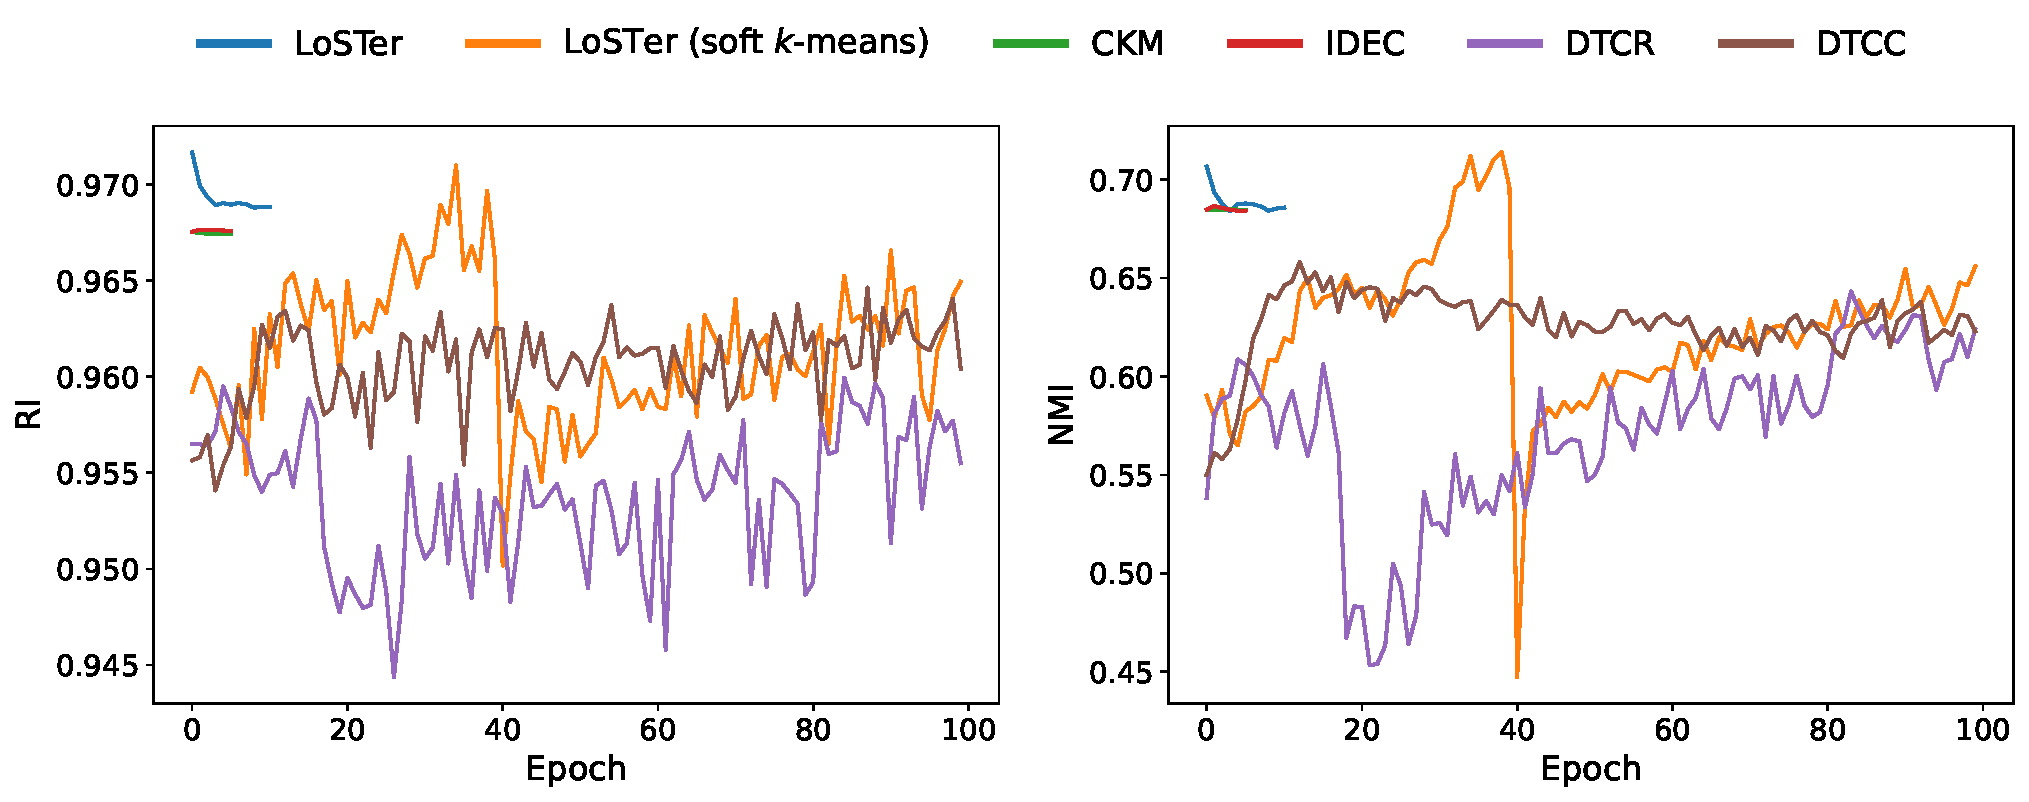
\includegraphics[width=\linewidth]{Figure_2.pdf}
  \caption{Rand Index (left) and Normalized Mutual Information (NMI) across the training process on NonInvasiveFetalECGThorax1.}
  \label{fig:convergence_NonInvasiveFetalECGThorax1}
\end{figure}

\begin{figure}[!htb]
  \centering
  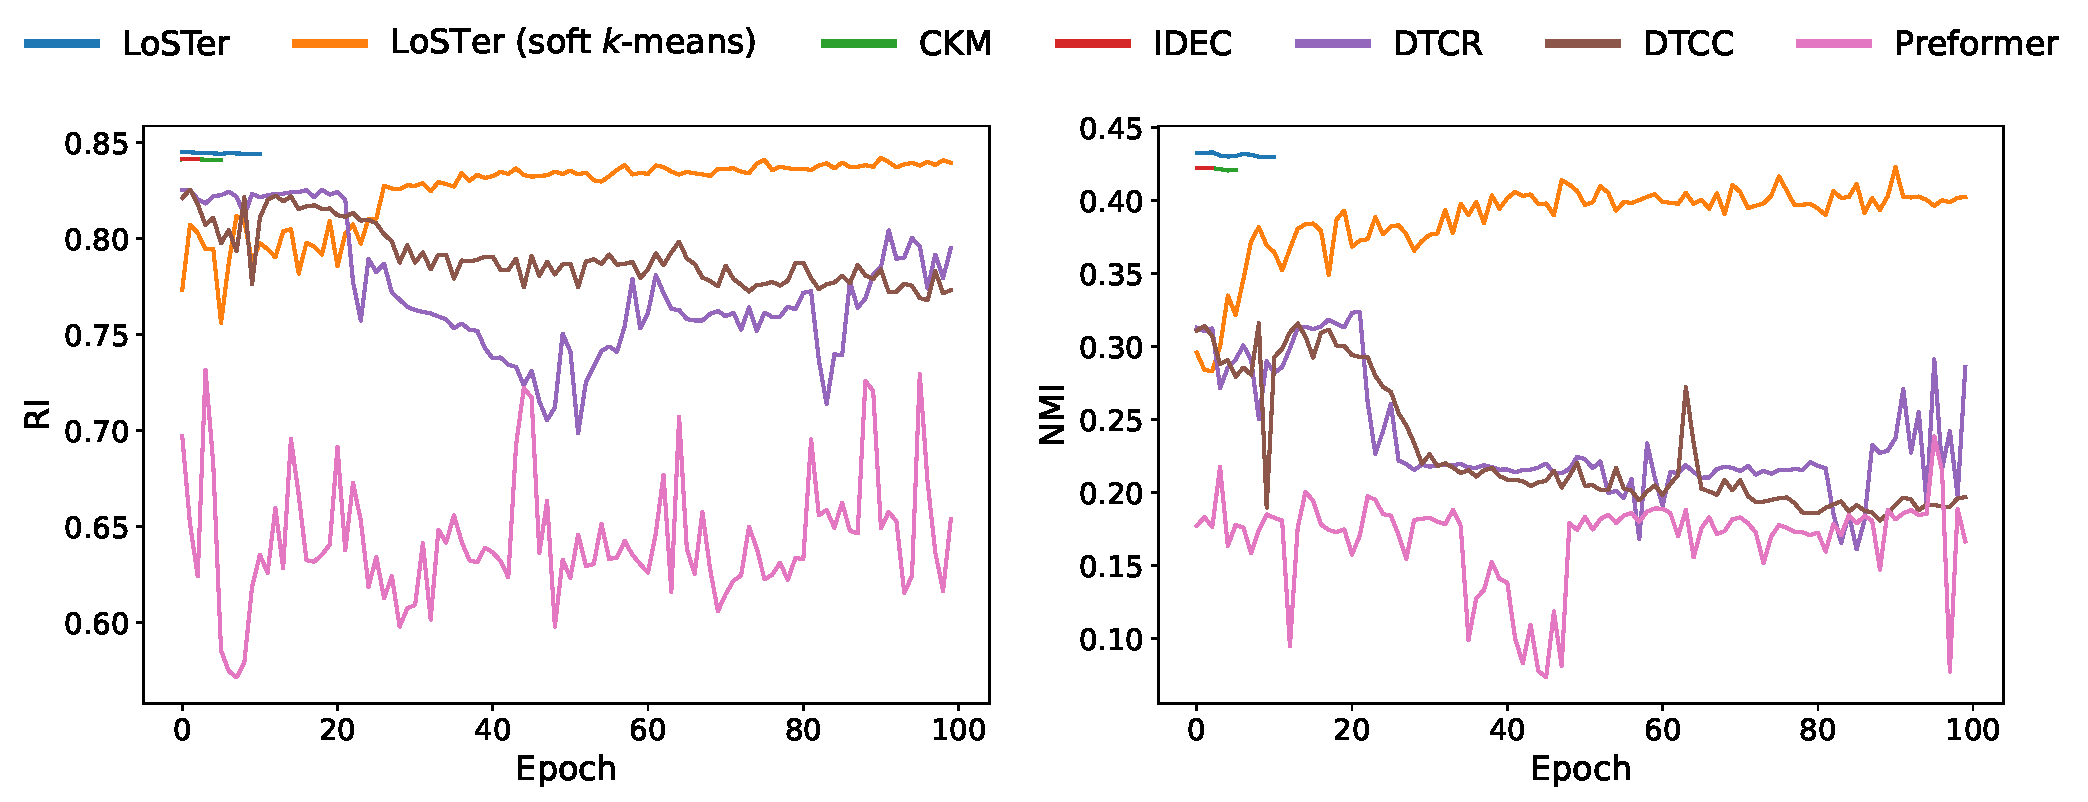
\includegraphics[width=\linewidth]{Figure_3.pdf}
  \caption{Rand Index (left) and Normalized Mutual Information (NMI) across the training process on UWaveGestureLibraryY.}
  \label{fig:convergence_UWaveGestureLibraryY}
\end{figure}

\textcolor{blue}{LoSTer shows rapid and stable convergence, achieving high RI and NMI scores within the first 20 epochs. This contrasts with DTCR and DTCC, which display high volatility in the metrics plots. Their reliance on autoregressive RNNs and fixed assignment updates leads to accumulated reconstruction errors and unstable learning dynamics. Unlike LoSTer, both DTCR and DTCC do not reach the point where less than 0.1\% of the samples change the cluster assignment between two consecutive epochs, indicating high fluctuation and lack of convergence, resulting in the completion of all 100 epochs. On the other hand, IDEC and CKM achieve better clustering performance with fewer epochs, approaching LoSTer's RI and NMI scores. This illustrates the drawbacks of soft \textit{k}-means optimization. Notably, the LoSTer variant trained with soft \textit{k}-means significantly outperforms DTCR and DTCC, highlighting the strength of the dense autoencoder compared to Dilated RNN architectures. However, with this variant, LoSTer must complete all training epochs, suggesting that while architecture plays a crucial role, optimization strategy remains a key factor in achieving fast and stable convergence.}

\textcolor{blue}{All models outperform Preformer regarding the UWaveGestureLibraryY dataset. Despite adopting the same Gumbel-softmax optimization as LoSTer, Preformer fails to converge and exhibits notable fluctuations throughout the 100 training epochs. This unstable behavior underscores the structural inadequacies of Transformer architectures for LSTC. As discussed previously, the permutation invariance of attention, the absence of semantic meaning of time points in time series, and the reduced batch size undermine the effectiveness of Transformers in capturing temporal dependencies. The failure of Preformer to capitalize even on advanced optimization strategies further reinforces the argument that Transformers, while effective in other domains, are fundamentally ill-posed for LSTC.}

\subsection{Large-Scale Time Series Clustering}
\begin{table}[!htb]
  \caption{Rand Index (RI) and Normalized Mutual Index (NMI) for real-world retail datasets. The best results are highlighted.}
  \label{large-scale-table}
  \vskip 0.1in
  \centering
  \resizebox{\linewidth}{!}{
  \begin{tabular}{lllllllll}
    \toprule
    Dataset & Metric & LoSTer & IDEC & DNFCS & CKM & DTC & DTCR & DTCC\\
    \midrule
    \multirow{ 2}{*}{M5} & RI & \textbf{0.8985} & \textbf{0.8985} & 0.8973 & 0.893 & 0.8914 & 0.8973 & 0.898\\
    & NMI & \textbf{0.1836} & 0.1705 & 0.1689 & 0.1678 & 0.111 & 0.1288 & 0.1368\\
    \midrule
    \multirow{ 2}{*}{Store Sales} & RI & \textbf{0.9523} & 0.9281 & 0.9247 & 0.915 & 0.9199 & 0.9116 & 0.9347\\
    & NMI & \textbf{0.4844} & 0.4298 & 0.4233 & 0.4216 & 0.2663 & 0.2354 & 0.2576\\
    \bottomrule
  \end{tabular}}
  \vskip -0.1in
\end{table}

In addition to common long-term benchmarks, we assess LoSTer on two challenging large-scale real-world retail forecasting datasets.

1) The M5 competition dataset contains 30490 time series with 1913 time steps recording the daily sales of items of different categories at Walmart in various stores, departments, and states over 6 years in the USA. However, M5 is a sparse dataset: since the many zero-sales days may impact clustering more than other sales characteristics, only 1150 time series are considered and we aim to group them into 29 clusters according to category and store.

2) The Store Sales competition dataset is used for predicting daily sales of thousands of products sold by different stores in the main cities of Ecuador over 5 years. Here, the scope is clustering 1729 time series of 1684 steps into 33 families of products.

RI and NMI scores are reported in Table \ref{large-scale-table}. Despite all models are comparable on M5 in terms of RI, LoSTer achieves a 0.1836 NMI score, which is higher than the 0.1705 of the runner-up IDEC. The margin is greater for the Store Sales dataset: the RI score by LoSTer is 0.9523 and higher than DTCC at 0.9347, while the NMI score is 0.4844 against 0.4298 by IDEC. Other models are less accurate.

\subsection{Training and Inference Speed}
\begin{figure}[!ht]
  \centering
  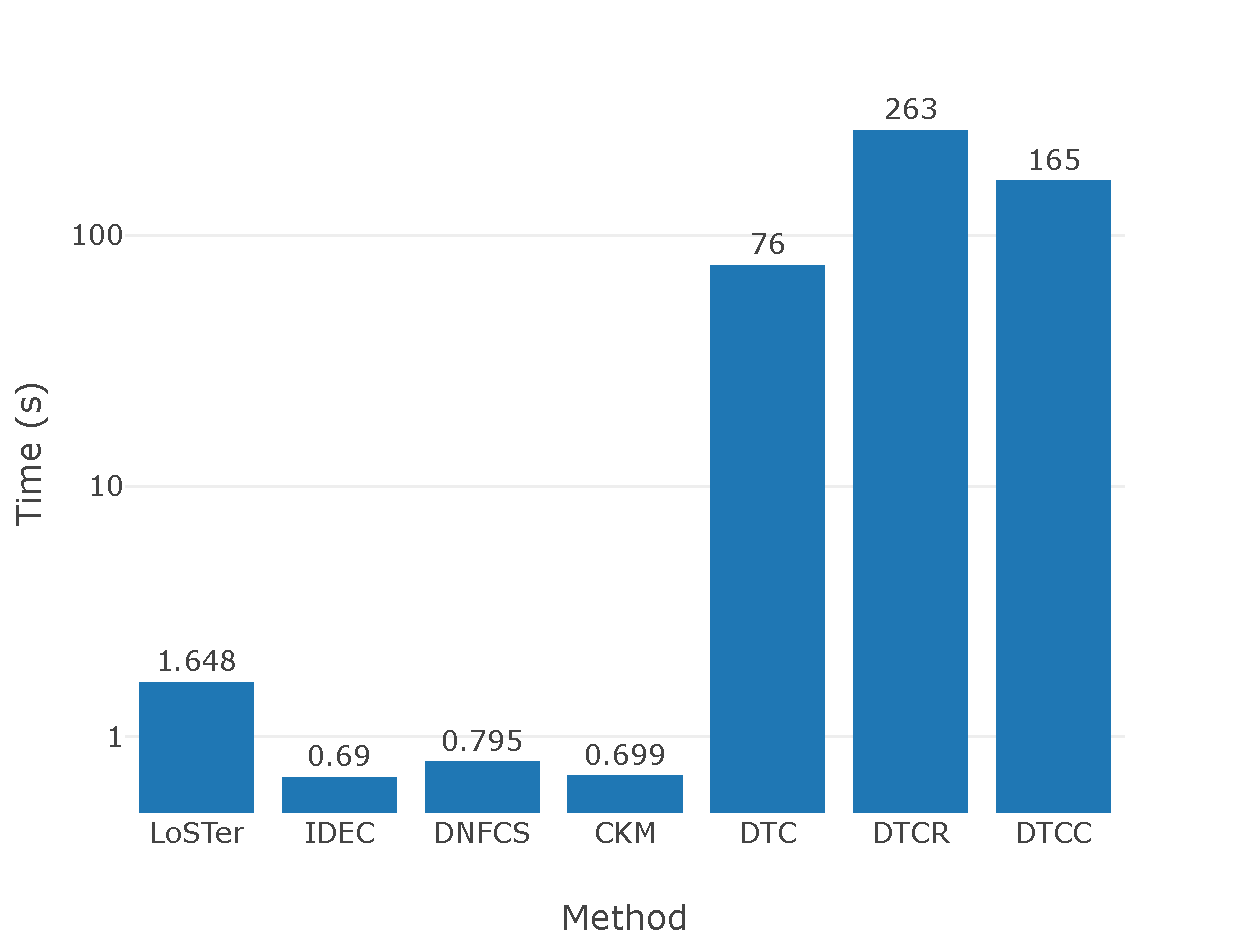
\includegraphics[width=0.8\textwidth,keepaspectratio]{Figure_4.pdf}
  \caption{\textcolor{blue}{Training times for one epoch by baselines to LoSTer for the Store Sales dataset plotted on a logarithmic scale to favor readability, as the fastest method (IDEC) and the slowest method (DTCR) are separated by 3 orders of magnitude. The actual running times (in seconds) are shown above each bar. RNN-based models such as DTCR and DTCC are significantly slower.}}
  \label{fig:training_efficiency}
\end{figure}

\begin{table}[!htb]
  \caption{Training and inference time for the StarLightCurves dataset.}
  \label{time-table-transformers}
  \vskip 0.1in
  \begin{center}
  \begin{small}
  \begin{tabular}{lll}
    \toprule
    Model & Train & Inference\\
    \midrule
    LoSTer & 2.85 s & 1.81 s\\
    Preformer & 1531 s & 270 s\\
    Pathformer & 550 s & 60 s\\
    iTransformer & 3.66 s & 2.03 s\\
    \bottomrule
  \end{tabular}
  \end{small}
  \end{center}
  \vskip -0.1in
\end{table}

MLP-based models enjoy faster training time than RNNs whose computations must be performed sequentially because the next output depends on the hidden state from the previous iteration. The single-layer RNN in the decoding phase of DTCR and DTCC limits severely the computing speed of the GPU, especially on long sequences. We demonstrate these effects by reporting in Fig. \ref{fig:training_efficiency} the average training times for one epoch in seconds on the Store Sales dataset with batch size 32. LoSTer completes one epoch in less than 2 seconds, which is lower by far than DTC (76 s), DTCR (263 s), DTCC (165 s) and still close to MLP competitors: IDEC (0.69 s), DNFCS (0.795 s), CKM (0.699 s). The simple yet effective dense architecture of LoSTer exhibits faster training than recurrent models. All running times are measured on a machine powered by a single NVIDIA A4000 GPU and 24 cores Intel(R) Xeon(R) CPU @ 2.40GHz.

Table \ref{time-table-transformers} reports the same time comparison for Transformer-based models in completing one training and one inference data pass of the StarLightCurves massive dataset. While the training and inference by LoSTer and iTransformer take around 3 seconds, Preformer and Pathformer require hundreds of seconds or more because of learning and then attending the many temporal tokens of input time series. Eventually, the RNNs and Transformers' computational complexity leads to longer training/inference times - in addition to poor clustering accuracy - making their real-world deployment infeasible for LSTC purposes.

\section{Conclusion}
This work presents LoSTer, a novel dense autoencoder architecture that addresses long-standing limitations in deep temporal clustering, particularly in the challenging setting of long-sequence time series clustering (LSTC). Current models attempting to incorporate the $k$-means objective into end-to-end training of neural networks need to rely on surrogate losses such as KL divergence or soft $k$-means approximations, which are known to be sub-optimal. These surrogates can cause overlapping and introduce unstable and inconsistent assignments when training through mini-batch stochastic gradient descent. To the best of our knowledge, this is the first study to thoroughly expose and address these drawbacks within an LSTC perspective.

In addition, our work is the first to provide a comprehensive critique of state-of-the-art RNN-based models in LSTC, identifying how their autoregressive decoding strategy leads to cumulative reconstruction errors and significantly slows training when dealing with long sequences. Equally, we discuss the shortcomings of introducing Transformers in this context. Despite their success in NLP and computer vision, standard Transformer architectures require specific adaptation to time series data due to the lack of semantic meaning in time points, the intrinsic permutation invariance which discards chronological order, and the quadratic computation and memory complexity of the attention mechanism. Notably, while forecasting requires predicting the next time steps for each input time series individually, clustering aims at partitioning a set of arbitrarily long sequences as a whole. The high memory occupation by Transformers forces to set a smaller batch size, thus affecting the final results, since clustering in deep learning is performed at the batch level. We emphasize that these limitations, which are exacerbated in LSTC, have not been explored yet.

In light of these observations and inspired by the recent success of simple linear models in long-term time series forecasting, the proposed method LoSTer leverages a stack of dense residual blocks in a dual contrastive framework to encode and decode time series efficiently while enabling differentiable optimization of the hard $k$-means objective using the Gumbel-softmax reparameterization trick. The architecture avoids autoregressive decoding, preserves temporal order, and allows for fast training and large batch processing. \textcolor{blue}{Eventually, this study demonstrates through extensive empirical validation on 17 benchmark datasets and two large-scale retail datasets that such a minimalistic design - free from recurrence and attention - can outperform state-of-the-art RNN and Transformer-based methods for LSTC.}

\subsection{Limitations and Future Works}
\textcolor{blue}{While LoSTer demonstrates significant advances in LSTC, the current study is limited to univariate time series. Future works include extending LoSTer to multivariate time series clustering, which remains an underexplored task, with a focus on benchmarking its accuracy, convergence, and speed against RNN-based and Transformer-based models. This involves assessing the impact of architectural choices - including seasonal-trend decomposition, and channel independence (i.e., processing each time series in the multivariate data separately, without blending or explicitly modeling interactions between them) versus feature mixing - to determine the most effective approach for capturing dependencies across multiple variables in complex real-world scenarios.}

\textcolor{blue}{Second, LoSTer does not focus on advancing the state of the art in contrastive clustering itself. Recent developments such as Cross-Domain Contrastive Clustering (CDCC) \cite{peng2024cross}, which leverages both temporal and frequency domains through cross-domain constraints, offer stronger mechanisms. Therefore, replacing dual contrastive learning in LoSTer with more sophisticated objectives represents a direction that could further enhance clustering performance. In this sense, LoSTer provides a strong foundation - through its differentiable hard clustering and dense residual architecture - upon which more advanced contrastive learning strategies may be integrated.}

\textcolor{blue}{Third, while LoSTer shows robust performance on two large-scale retail datasets, validation in other domains such as healthcare, IoT, or finance may further demonstrate its generalizability.}

By bridging architectural simplicity with an innovative optimization strategy, we hope LoSTer will guide upcoming studies in time series clustering and prompt broader reconsideration of model complexity in deep learning for temporal data.

\section*{Acknowledgements}
This work has been partially supported by the European Union under the Italian National Recovery and Resilience Plan (NRRP) of NextGenerationEU, partnership on “Telecommunications of the Future” (PE00000001 - program “RESTART”) focused project WITS and project “Rome Technopole” PNRR-NextGenerationEU n. ECS 00000024, Mission 4 Education and Research, Component 2 From Research to Enterprise, Investment. 1.5 Creation and strengthening of “Innovation ecosystems for sustainability”.

%% The Appendices part is started with the command \appendix;
%% appendix sections are then done as normal sections
%\appendix

%% If you have bib database file and want bibtex to generate the
%% bibitems, please use
%%
\bibliographystyle{elsarticle-num}
\bibliography{biblio}

\end{document}

\endinput
%%
%% End of file `elsarticle-template-num.tex'.
